\documentclass{beamer}

\usepackage{beamerthemesplit}
\usepackage{graphicx}

\usetheme{Berlin}
\usecolortheme{albatross}

\author{Daniel Johnson}
\title{A Distributed Multicast DNS System}
\begin{document}
\section{Overview}
\frame{\titlepage}
\section{Purpose}
\frame{
\frametitle{Purpose and Scope}
To allow a group of workstations as present on a medium-size subnet to survive complete loss of a DNS server through collaboration. The syslab workstations provide an example of an appropriate size.
}
\section{Background}
\frame{
	\frametitle{Background Research}
Several efforts have been made to solve similar problems:
	\begin{itemize}
	\item The Apache project provides name lookups for machines on the local subnet vial a .local pseudo-TLD
	\item DistributedDNS attempts to surpass the traditional ICANN-based name service, which is too ambitious to succeed.
	\end{itemize}
	My solution with work with the local link only, which will keep speed as fast as or faster than traditional nameservers, provide lookups for all hosts, not just nearby ones, and honor the authority of the root nameservers.

Another important algorithm may be DHT: Distributed Hash Tables. Since DNS records are key-value pairs, this may be perfect.
}
\section{Tools}
\frame{
\frametitle{Computer Language/Software}
Python is being used for prototyping and network simulation. Eventual client/server will be written in C++.
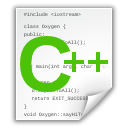
\includegraphics{text-x-c++src.png}

\includegraphics{text-x-python.png}
}
\section{Procedure}
\frame{
\frametitle{Procedure}
\begin{itemize}
	\item Python
	\begin{itemize}
		\item Proof-of-concept
		\item Protocol development
	\end{itemize}
	\item C++
	\begin{itemize}
		\item Client/server development
		\item Name Service Switch (NSS) module
	\end{itemize}
\end{itemize}
}
\section{Analysis}
\frame{
\frametitle{Testing/Analysis}

\begin{itemize}
	\item Simulation tests
	\begin{itemize}
		\item Network chatter
		\item Protocol development
		\item Degradation of network
	\end{itemize}
\end{itemize}
}
\section{Results}
\frame{
\frametitle{Expected Results}
The benefits of offloading routine and emergency duties from the nameserver has several practical benefits. First, in the event of a nameserver outage, not all systems need to fail. While non-cached entries may not be available, those that have seen high use (google.com, for example) will still be available. This helps to eliminate one instance of a single point of failure. With a sufficient number of hosts, processing queries on the main nameserver can lead to performance issues. By dividing responsability for name lookups among hosts, the speed and scalability of lookups can be improved.
}
\end{document}
